% Resultater

\chapter{Resultater} % Chapter title

\label{ch:resultater} % For referencing the chapter elsewhere, use \autoref{ch:resultater}

%----------------------------------------------------------------------------------------

% Skrives i fortid.

I dette kapittelet blir resultater som har kommet frem i løpet av prosjektperioden presentert. Gruppen har blant annet tatt personlighets\-test og en felles øvelse om samarbeid, i tillegg til å skrive personlig logg underveis i prosjektperioden. Her kommer det frem hvordan gruppen har utviklet og tilpasset seg i forhold til resten av gruppen.

% Personlige refleksjoner / Forholdet til EiT / Hva dere har lært som enkeltpersoner. 

% Sees f.eks. opp mot hva som ble presentert om hver enkelt i innledningen. Dette er tema hvor vi sensorer ikke kan sammenligne dere med forventninger, sammenligne dere med hverandre, eller sette karakter på dere. Det er flott hvis det kommer frem noe interessant, men ikke gjør slike kapitler til pliktløp, og (vær så snill!) ikke lag kapitler fylt med svada.

\section{Personlighetstyper og roller i gruppen}

Omtrent halvveis gjennom prosjekttiden hadde vi en rolleøvelse i gruppen. Hensikten med denne øvelsen var å bevisstgjøre hverandre på hvilken rolle hver enkelt av oss hadde. Grafisk fremstilling av øvelsen kan sees i \autoref{ch:roller}, der hver figur tar for seg poengene som én person fikk, inkludert personens poeng til seg selv.

På eget initiativ gjennomførte gruppen den velkjente <<Myers-Briggs Type Indicator>>-testen for å kartlegge hvilke personlighetstyper gruppen besto av. Vi endte opp en ENFJ, en ENFP, en ISFJ og tre ISTJ.

I rolleøvelsen kom det klart frem at alle i gruppen så på gruppemedlemmet med ENFP personlighet som den personen som tok mest ledelse og generelt satt mye preg på gruppen. Samme gruppemedlem kom også klart ut som den i gruppen som var minst underkastende og som utfordret andres ideer mest. En person med ENFP personlighet er sosial, nytenkende og opptatt av harmoni og godt samarbeid i gruppen, og passer derfor ofte godt som leder. Dette gruppemedlemmet var også gruppens eneste oppfattende person og er derfor mer opptatt av prosessen enn målet. Selv om resultater selvsagt er viktig for en leder, så kan for stort fokus på resultatet føre til hastet arbeid av dårlig kvalitet. Derfor bør ofte en god leder være opptatt av prosessen, noe som styrker vår tro om at riktig person opptrådte som leder i gruppen vår.

Vi hadde et tydelig skille i personlighetstyper i gruppen vår. På ene siden hadde vi en av type ENFJ og en av type ENFP som er utadvente, nytenkende og opptatt av godt samarbeid. På andre siden hadde vi tre av type ISTJ og en av type ISFJ som gjerne er litt mer stille, faktaorienterte og målrettet. I øvelsen kom det frem at de to med ekstroverte personlighet var de som tok mest av gruppens oppmerksomhet, både på godt og vondt. De introverte var jevnt over dem som i øvelsen som scoret høyest på å innordne og underkaste seg, være taus eller stille. Dette resultatet kom ikke som noe overraskelse på gruppen, siden det ligger langt mer i en ekstroverts natur å være gruppens midtpunkt, enn hva det gjør for en introvert.

Når det kom til hvem i gruppen som var sosial og bidro til å skape hygge og trivesel, fikk alle i gruppen god score. Likevel pekte gruppemedlemmet med ENFJ personlighet seg ut som den mest sosiale, og som bidro mest til trivselen i gruppen. Dette er en rolle som ofte faller naturlig for en med ENFJ personlighet. 

Øvelsen viste oss også at alle i gruppen hadde gitt ganske lik poengsum til seg selv som det de andre i gruppen hadde gitt en. Det viser at våre oppfatninger av oss selv i gruppen samsvarer med andres oppfatninger. Vi tror at ved å ikke ha noen vrangforestillinger av våre egne roller i gruppen, så har vi unngå en del konflikter som ellers kanskje ville oppstått.

\section{Samarbeidsindikatoren}
I løpet av prosjektperioden ble det tatt en undersøkelse tre ganger; en ved start, midten og ved slutten av prosjektet. Resultatet viste i hvilken grad disse faktorene ble nådd, se \autoref{samarbeidsindikatoren}. Ser på figuren at resultatene stort sett sank utover i perioden. Det er viktig å merke seg at to forskjellige gruppemedlemmer var borte henholdsvis andre og tredje gangen. Vi tror dette har påvirket resultatet, særlig tredje gangen. 
\begin{figure}[!h]
    \centering
    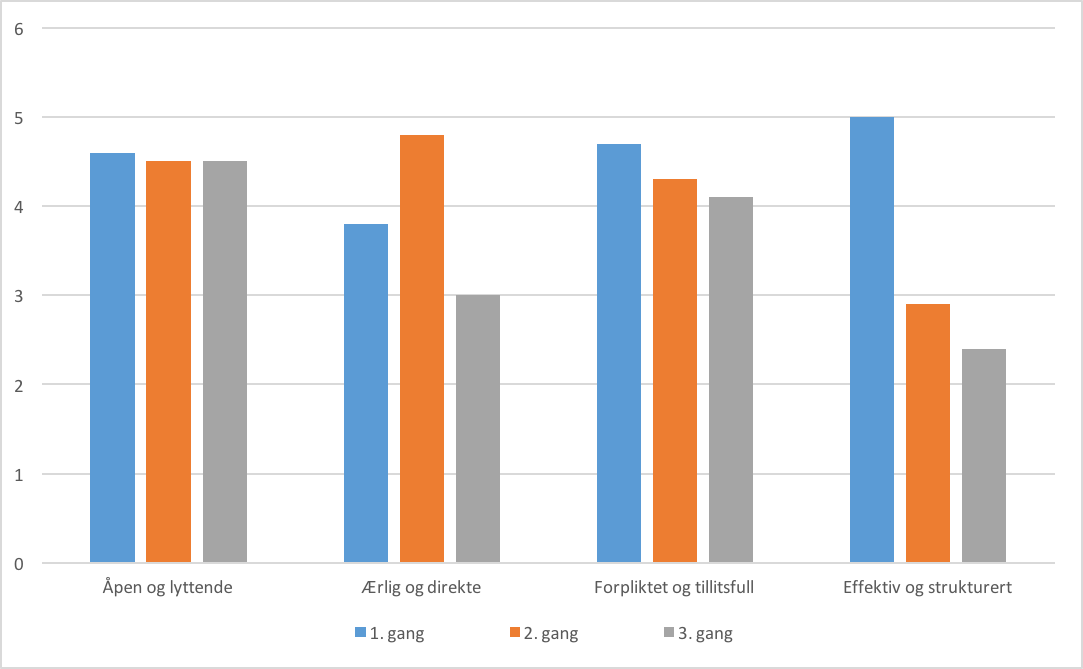
\includegraphics[width=1\textwidth]{gfx/samarbeidsindikatoren.png}
    \caption{Samarbeidsindikatoren}
    \label{samarbeidsindikatoren}
\end{figure}

Hvis vi fokuserer på <<Ærlig og direkte>>, så har den sunket den gangen den mest direkte personen på gruppen var borte. Dette må være grunnen til at den har sunket til der den endte. Vi mener selv at vi alltid har vært like ærlige og direkte mot hverandre, selv om figuren kanskje ikke viser det. I løpet av perioden har effektiviteten kanskje gått litt ned i perioder. I starten kom gruppen godt i gang og var produktive. Da den andre undersøkelsen skulle tas var vi litt skuffet og ikke fornøyd med hvor langt vi hadde kommet i forhold til målet med prosjektet, derav lavt resultat på <<Effektiv og strukturert>>. Gruppen hadde fått litt mer motgang enn forventet. For noen gruppemedlemmer forsvant ikke denne motgangen og påvirket også den tredje undersøkelsen. Personen som var borte tredje gangen var han som jobbet mest med det tekniske og hadde vært mye mer effektiv og produktiv enn hva de andre på gruppen fikk inntrykk av. Siden de fleste på gruppen hadde lite å gjøre med det tekniske utover i prosjektperioden, følte de at de ble mindre effektive, selv om de fikk jobbet mye med rapportene eller andre ting som kunne være til hjelp for prosjektet. Vi mener dette senktet den oppfattede effektiviteten og kunne realistisk sett ligget et sted mellom første og andre gang. 

Hvis man sammenligner gruppens arbeid mot Roger Schwarz sin bok om fasilitering, i kapittelet <<What Makes Groups Effective>> \cite[s. 17-34]{schwarz_skilled_2002}, er det flere sammenhenger som tyder på at effektiviteten i gruppen ble slik som resultatet viser. I starten var gruppen mer definert med hver sine oppgaver, det var et tydelig mål, alle var motivert og følte eierskap til problemstillingen. Etter å ha byttet idé et par ganger ble det målet som i starten var felles, mer en person sitt mål som resten av gruppen fulgte. Dette var mindre motiverende for resten av gruppen når de ikke lenger var like mye med på målet gruppen hadde satt seg. Dette førte til mindre gruppestruktur og resulterte i lavere effektivitet. 

\section{Personlige refleksjoner}
\subsection{Jon}

% Gruppedynamikk har fascinert meg lenge, spesielt etter jeg skrev bacheloroppgave i 2013. Vi var tre gutter som jobbet sammen, hvorav de to andre på gruppen kjente hverandre fra før. Vi leverte et godt resultat, men veien dit var fylt med personlige konflikter, dårlige tilbakemeldinger og uheldige forsvarsmekanismer. Dette er ting jeg på den tiden tenkte mye over, som jeg merket ødela for motivasjonen til arbeidet, og som kunne gjort prosjektet enklere hvis jeg og de andre på gruppen hadde oppført oss annerledes. Videre ble jeg ble spurt om hva slags grupperolle jeg tar under et jobbintervju senere i 2013. Jeg føler jeg svarte godt for meg på tidspunktet, men skjønte senere at jeg ville lære mer om dette da jeg hørte hva EiT gikk ut på. Ellers kan kunnskapen brukes i det personlige livet, enten i familie, bofellesskap eller med kjærester. 

% Etter fem år med høyere utdanning preget av mye gruppearbeid har jeg begynt å se trender på hva slags rolle jeg tar i grupper. Under EiT har jeg hatt forventninger til å sette ord på flere av disse trendene, bli mer kritisk til hva jeg kommuniserer både med det jeg sier og det jeg ikke sier, og å lære om hvilke handlinger som er rette å gjøre i dilemmaer hvor to sider av en konflikt har gode poeng om hvorfor de har rett. 

Jeg ser på meg selv som en utadvent person, og dette har også blitt bekreftet fra inntrykk jeg har mottatt i gruppen. Det var viktig for meg å bli kjent med alle i gruppen fra starten, spesielt siden jeg gikk glipp av første landsbydag. Det er den sosiale rollen jeg etterhvert festet i gruppen jeg føler er mest interessant å reflektere over. Den sosiale rollen er et produkt av at jeg engasjerer meg med innspill i diskusjoner om arbeid, gir tilbakemeldinger, er en god lytter, opptatt gruppemedlemmers velvære og er en bidragsyter under pauser og i lunsjen. Jeg prøver å ha fokus på å få med alle, det betyr for eksempel at jeg eksplisitt spør de minst deltagende om deres mening. Til tross for dette er det noen jeg har fått bedre kontakt med på gruppen, som jeg automatisk gir litt mer oppmerksomhet. Jeg synes det er viktig å balansere ris og ros, og har fokus til på å bidra mot dette. Dette er noe som funker mye i mitt daglige liv, som jeg har fortsatt med i prosjektarbeidet og gjennomført i varierende mengde. Ros øker mestringsfølelsen til mennesker, og kan virke motiverende. I praksis er det ofte enklere å kritisere noen for noe de har gjort feil eller ikke gjort, heller enn noe som oppfyller forventninger eller er gjort bra.

En betydelig bieffekt av rollen min i gruppen er at jeg tar opp mye oppmerksomhet. Dette er selvsagt på godt og vondt, men sett over hele prosjekttiden har det nok vært mest negativt. I startfasen mens vi diskuterte problemstilling kunne jeg fort gi et ironisk svar på idéer som uansett kanskje virket litt for oppfinnsomme. Denne ironien kunne så bli misforstått som videre førte til bortkastet tid. Jeg er nok også en av de i gruppen som bidrar til flest avsporinger. Selv om flere enn meg skal ha skyld for unødvendige avsporinger, sitter jeg med en følelse av at jeg har brakt frem en evne til hyppigere avsporinger hos mennesker som vanligvis kanskje ikke sporer av så ofte. Dette er en interessant karakteristikk, og noe jeg tar med meg videre. Som følge av dette burde jeg se an situasjonen og generelt forholde meg helt seriøs, og spare vitser, historier og andre temaer som ikke passer under arbeid til lunsj og pauser. Dette er det viktig at jeg får endret på.

En annen konkret atferd som har hatt noe å si for gruppa er mengden tid jeg bruker på å være for sen. Jeg kommer ofte fem minutter for sent til arbeidsdagen, og dette forsinker ikke bare gruppa til rommet hvor vi skal jobbe, men det kan også skape irritasjon eller forstyrre arbeidspsyken som noen bygger seg opp. Bakenliggende årsaker for at jeg kommer for sent til arbeidet når jeg klarer å rekke busser, jobb og andre litt mer definerte avtaler og obligatoriske tidspunkt kan være fordi jeg ikke prioriterer arbeidet nok i hodet mitt. I tillegg finnes det rom i reglene som ikke straffer mindre forsinkelser. Forsinkelsene mine har blitt tatt opp flere ganger i gruppa, og jeg ønsker å bli flinkere på dette, og burde lære meg å gi tilsvarende settinger høyere prioritet.   

Når det kommer til arbeid med prosjektet er jeg fornøyd med egen innsats, mindre fornøyd med egen konkret leveranse. Jeg tok tidlig på meg ansvaret for dokumentasjon og papirer, som en slags sekretær i gruppa. Dette var også i henhold til samarbeidsavtalen. Jeg skrev mesteparten av grupperefleksjonene, men var til stadighet ikke helt fornøyd hvordan de ble sammenlignet med eksempelrefleksjonen. Videre prøvde jeg hele tiden å engasjere meg i arbeidsoppgaver hvis jeg ikke hadde noe å gjøre. Eksempelvis prøvde jeg å paralellisere arbeidet i større grad ved å få opplæring og bidra med mine kunnskaper i programmering, men det viste seg at det ble vanskelig på grunn av feilmeldinger og bugs som oppstod. Da falt jeg tilbake på å skrive rapport eller lese teori. 

Jeg er fornøyd med måten jeg møter kritikk på, spesielt i en setting som EiT. Hvis mennesker gir tilbakemeldinger på en konstruktiv måte er jeg veldig tilbøyelig for å høre på og ta det til meg. Mitt mål er å bli verdsatt av gruppemedlemmene mine, slik at de kan ha tillit til å delegere arbeid til meg, eller ta på seg arbeid for meg.

\subsection{Harald}
Da jeg først fikk vite om emnet Eksperter i Team ble jeg interessert i hvilken landsby jeg ville ende opp og hvem jeg kom til å jobbe sammen med en gang i uken i løpet av et semester. Jeg fikk den samme følelsen som jeg har fått når jeg skal begynne i en ny klasse på en ny skolen, det var litt spennende. I starten av prosjektperioden var jeg motivert til å lære mye om meg selv i en gruppesammenheng i tillegg til å utforske muligheter rundt temaet om roboter i samfunnet. Førsteinntrykket til Eksperter i Team var bedre enn forventet. Siden jeg er en anelse sjenert, særlig rundt nye mennesker, var jeg litt stille i starten. Dette var også fordi noen andre på gruppen hadde en tendens til å prate mye, og førte til at jeg ikke helt kom på samme plan som andre i gruppen. Etter noen ganger fikk gruppen balansert seg litt og samtalen ble bedre fordelt utover flere parter. 

En ting som jeg angrer litt på er at jeg ikke satte meg mer inn i det tekniske på starten. Siden det var ukjent og andre på gruppen hadde kommet mer igang, trakk jeg meg litt tilbake og lot andre jobbe med det. Dette førte til at jeg gikk glipp av muligheten til å arbeide med det tekniske. Noe jeg har merket mer prosjektarbeid i gruppe er at jeg kanskje bryr meg mer om å møte opp og være tilstede enn å være produktiv. Jeg følte til tider at jeg ikke fikk gjort så mye som jeg burde. Dette har også litt med det at vi hadde udefinerte arbeidsoppgaver. Utover i perioden lot jeg meg kanskje irritere litt over småting, som at noen ofte var sene om morgenen. Det var lett å glemme slike små ting når man ser på helheten. Jeg var generelt veldig fornøyd med samholdet i gruppen, og føler jeg har lært mer om hvordan jeg fungerer i et team.

\subsection{Erlend}
Jeg hadde egentlig ikke så mange forventninger når jeg begynte med Eksperter i Team. Landsbyen jeg havnet i, Robotikk og Menneske, var andrevalget mitt. Førstevalget var byggelandsbyen, dette fordi jeg generelt liker å jobbe med praktiske ting. Jeg hadde hørt fra andre om at kvaliteten på emnet i hovedsak var avhengig av hvilken gruppe en havnet på. Derfor var det gledelig at jeg allerede fra første dag hadde et positivt inntrykk av de jeg kom på gruppe med. Jeg likte det faktum at vi var en ren teknisk gruppe med forholdsvis like studie\-retninger. Jeg så på dette som en fantastisk mulighet til å kunne lage noe spennende sammen. Personene på gruppen virket også engasjerte og motiverte i forholdet til emnet. Samtalen fløt også lett, og det var ikke noe problem med å få sagt sin mening til en hver tid. 

Selv så har jeg aldri betraktet meg selv som en lederperson. Samtidig så har jeg heller aldri har vært avhengig av at folk må fortelle meg hva jeg skal gjøre til en hver tid. Jeg liker å delta aktivt i de avgjørelsene som blir tatt, og ikke bare passivt si meg enig i det andre mener er den beste avgjørelsen. Jeg har derfor på flere tidspunkt i løpet av dette emnet vært i opposisjon på en del store avgjørelser. Nå i ettertid ser jeg at dette er en rolle som jeg kunne ha inntatt i enda større grad. Jeg kom nemlig med en god del kritikk til å bruke Motion-Capture systemet i forbindelse den autonome handlevognen. Jeg påpekte at tiden for gjennomføre et slikt prosjekt var for liten, og at oppgaven dårlig lot seg dele opp. Nå i ettertid har det vist seg at mitt sistnevnte argument har vært et stort problem for gruppen. Oppgaven vi landet på var vanskelig å dele opp, noe som førte til at effektiviteten gikk betydelig nedover. 

Rent jobbmessig så er jeg helt greit fornøyd med min egen innsats. Jeg er kun misfornøyd med at jeg ikke har fått bidratt så mye med det jeg er virkelig god på. Eksperter i Team har først og fremst lært meg hvor viktig det er å ytre sin mening, spesielt hvis det er noe man sitter å brenner inne med. Dine argument er vel så gode som alle andres, og det er derfor så utrolig viktig å få diskutert dem. 

\subsection{Håvard}
Jeg gikk inn i Eksperter i Team med positive forventning og var veldig spent på hvordan jeg kom til å fungere med en helt ny gruppe mennesker. Opp i gjennom studietiden har jeg vært bundet til grupper jeg allerede kjente fra før, så å kunne møte nye folk i en helt ny gruppe ville bli spennende. Jeg har en veldig skeptisk og realistisk holdning, dette var noe jeg håpet ikke ville være i veien for andre hvis de prøvde å strekke seg etter noe jeg mente var urealistisk. Men dette var ikke noe problem i vår gruppe da alle delte denne samme holdningen. Jeg er vant med å måtte lede litt, eller ihvertfall å få folk litt i gang med oppgaver, men denne gangen var jeg den som trengte å bli litt satt i gang. Dette var en helt ny erfaring for meg, og var veldig interessant. Jeg har følt at jeg har blitt bedre kjent med meg selv. Jeg fikk også oppleve at mitt humør kan gå ut over andre, og dette er noe jeg har prøvd å jobbe med mer i ettertid. Rent jobbmessig er jeg ikke spesielt fornøyd med egen innsats, jeg føler jeg kunne ha vært litt mer frempå slik at det kunne blitt mindre jobb for andre. Dette er noe vi har reflektert mye over mot slutten og blitt enig om at kunne vært annerledes. Alt i alt er jeg fornøyd og synes dette har vært en lærerik erfaring og ta med seg videre i livet og inn i arbeidslivet.

\subsection{Helene}
Jeg hadde allerede fra starten en positiv holdning til emnet. Jeg var spent på hvem jeg kom til å komme på gruppe med, men tenkte at emnet kom til å bli anderledes og interessant uansett. Gjennom mine fire år her på NTNU har jeg hatt mye gruppearbeid, likevel har jeg, som mange andre, ofte jobbet med de samme personene hver gang. Dette har gjort at jeg jobber veldig bra sammen med disse, men har fått lite trening å å forholde meg til nye mennesker. Jeg har heller ikke særlig erfaring med å jobbe i grupper på størrelsen med den vi har hatt i dette emnet. Jeg syns Eksperter i Team gir en mer realistisk opplevelse av hvordan et gruppearbeid foregår i arbeidslivet, noe jeg setter stor pris på å få øvd meg litt på. Jeg sitter igjen med følelsen av å ha lært mer om min innvirkning på en gruppe og at jeg vet mer om hva jeg kan gjøre for å bidra til å få et så effektivt gruppearbeid som mulig. Det har vært fint å hatt et emne hvor man har tid til å reflektere over gruppearbeidet og ikke bare haste i mål. Jeg tror jeg kommer til å få bruk for erfaringene jeg har fått gjennom Eksperter i Team når jeg kommer ut i arbeidslivet. 

Faglig føler jeg meg helt klart sterkest på teori og følte derfor ikke jeg hadde så veldig mye å bidra med på det praktiske som ble gjort. Likevel følte jeg at jeg var flink til å finne andre oppgaver som jeg var mer komfortabel med å gjøre. Jeg er derfor fornøyd med egen arbeidsinnsats.

\subsection{Morten}
Landsbyen, Robotikk og Menneske, var for min del andrevalget jeg søkte på. Jeg gikk likevel inn i emnet med åpent sinn, og forventning om at vi kunne få til noe interessant og givende. Tidlig i arbeidet følte jeg at vi hadde fått satt sammen en god gruppe, med komplementerende personligheter og erfaringsgrunnlag.

I gruppen tok jeg ganske tidlig en noe ledende rolle. Vi ble enige om å benytte tankegang fra såkalt smidig utvikling, eller Scrum\footnote{\url{http://en.wikipedia.org/wiki/Scrum_(software_development)}}, der man benytter seg av korte utviklingsintervall og tydelig definerte delmål. I dette paradigmet har man en <<Scrum Master>>, som har som rolle å fjerne utvendige hindringer som står i veien for gruppens fremgang, og generelt fungere som en buffer mellom gruppen og ytre forstyrrelser, i tillegg til å sørge for at gruppen har tilstrekkelig fremgang til å møte de kravene som stilles av ledelsen. Personen har ingen formell autoritet, men har en rolle som er beskrevet som en blanding av å være både gruppens leder og tjener, samtidig som man også arbeider med oppgaver på linje med de andre i gruppen. Dette har vært en ny rolle for meg, noe som har vært spennende. Det har derfor vært en god trygghet å kontinuerlig få tilbakemelding fra resten av gruppen om hvordan de har opplevd min rolle.

Som en følge av denne rollen har jeg i blant brukt ekstra tid for å sette meg inn i problemer som har vært til hinder for gruppens fremgang. En konsekvens av dette er at jeg har sittet på kompetanse ingen andre i gruppen har hatt. Vi har brukt noe tid på å spre denne kunnskapen, men kanskje ikke nok. Som en konsekvens føler jeg at gruppens effektivitet innen enkelte oppgaver har vært litt for avhengig av om jeg har vært tilstede eller ikke. Dette er nok en utfordring man møter i mange arbeidssituasjoner, og jeg skulle nok likt å vite mer om hvordan man håndterer det på en god måte.

Rollen jeg beskriver ovenfor, i sammenheng med at jeg er en forholdsvis utadvendt person, har ført til at jeg har vært fremtredende i diskusjonene i gruppa. Dette er noe det er viktig for meg å være bevisst på, slik at også de som ikke er like på hugget til å ta ordet får komme til. Emnet har gitt meg nyttig trening i nettopp dette. Ingen i gruppa har gitt meg tilbakemelding på at de har følt seg overkjørt, heller ikke på direkte spørsmål, og det tar jeg som en indikasjon på at jeg har funnet en god balanse.